\section{提出的方法}
\label{sec:proposed_approach}

我们提出了一种简单而高效的管道,AirRoom,用于房间重新识别,利用多层次的面向对象信息,如\fref{fig:pipeline}所示。接下来,我们将按照执行阶段的顺序系统地介绍管道的每个模块。
\subsection{全局阶段}

在此阶段,我们利用全局特征提取器捕获全局上下文特征,这些特征来源于房间内物体的集体存在。这些特征随后用于全局检索,从数据库中粗略地选择语义相似的候选房间。
\subsubsection{全局特征提取器}
\label{sec:section3.1.1}

与户外环境相比,室内房间的变化较少。它们缺乏多样的地形特征,如空中、地下或水下特征,也不经历像昼夜或季节性变化这样的时间性变化。因此,为每个室内房间收集大规模数据集是具有挑战性的,这使得许多视觉定位和重识别(VPR)方法的规模化训练变得复杂 \cite{arandjelović2016netvladcnnarchitectureweakly, hausler2021patchnetvladmultiscalefusionlocallyglobal, alibey2023mixvprfeaturemixingvisual}。

然而,室内房间本身在物体上具有丰富的多样性,每个物体都对房间的整体语义上下文做出贡献。通过利用这种全局上下文信息,我们可以将参考搜索专门集中在与查询图像具有相似语义特征的房间上。为此,我们倾向于选择在大规模图像数据集上预训练的骨干网络,因为它们提供了较强的泛化能力,能够有效地捕捉有价值的全局上下文特征 \cite{kornblith2019betterimagenetmodelstransfer}。因此,我们的模型选择包括基于卷积神经网络(CNN)的预训练模型,如 ResNet \cite{he2015deepresiduallearningimage},以及基于变换器的自监督学习模型,如 DINOv2 \cite{oquab2024dinov2learningrobustvisual}。
\subsubsection{全局检索}

使用全局特征提取器,我们为\(M\)个查询图像和\(N\)个参考图像提取全局上下文特征。令\(\mathbf{Q} \in \mathbb{R}^{M \times D_g}\)和\(\mathbf{R} \in \mathbb{R}^{N \times D_g}\)分别表示查询特征和参考特征,其中\(D_g\)是特征维度。然后计算余弦相似度矩阵\(\mathbf{S}\)为:
\begin{equation}
    \mathbf{S}_{ij} = \frac{\mathbf{Q}_i \cdot \mathbf{R}_j}{\|\mathbf{Q}_i\| \|\mathbf{R}_j\|}.
    \label{eq:global feature cosine similarity}
\end{equation}
对于每个查询,我们使用以下公式选择前5个最相似的参考候选:
\begin{equation}
    \text{Top}_5(\mathbf{S}_{i, :}) = \text{argsort}(-\mathbf{S}_{i, :})[:5],
    \label{eq:global retrieval}
\end{equation}
其中\(\mathbf{S}_{i, :}\)表示第\(i\)个查询的余弦相似度。
\subsection{局部阶段}

全局上下文特征提供了有价值的语义信息,有助于缩小候选列表的范围。然而,当面对许多语义相似的房间时,仅依赖全局上下文是不够的,局部特征变得越来越重要。在此阶段,我们采用局部视角,首先应用实例分割和感受野扩展器来识别物体和图像块。随后,我们使用物体特征提取器从物体和图像块中提取特征,接着通过面向物体的评分进一步优化候选列表。
\subsubsection{实例分割}

对于每张查询图像及其对应的五个候选图像,我们采用实例分割方法,如 Mask R-CNN \cite{he2018maskrcnn} 和 Semantic-SAM \cite{li2023semanticsamsegmentrecognizegranularity},来识别并描绘出各个独立的物体。该过程会生成每个物体的掩码和边界框。接下来,我们利用边界框计算每个物体的中心点 \(c\),如下所示:

\begin{equation}
    c = (\frac{x+W}{2}, \frac{y+H}{2}).
    \label{eq:center point}
\end{equation}

在此公式中,\(x\) 和 \(y\) 表示边界框左上角的像素坐标,而 \(W\) 和 \(H\) 分别表示边界框的宽度和高度。
\subsubsection{感受野扩展器}

单个物体的信息本身并不足以具有良好的判别性。例如,尽管不同的书桌可能具有不同的外观,它们既可能出现在食堂中,也可能出现在办公室中。然而,当一个物体与其邻近物体(如与计算机、键盘或笔记本并列的书桌)相关联时,就暗示该房间更有可能是办公室而不是食堂。这一见解促使我们将感受野从单一物体扩展到包含多个物体的图像区域。

给定图像中所有物体的中心点,我们采用 Delaunay 三角剖分法 \cite{10.5555/1370949} 来生成物体关系的三角形图。具体而言,Delaunay 三角剖分作用于物体中心点集合,确保没有任何物体中心位于任意三角形的外接圆内部。该方法最大化三角形的最小角度,避免出现狭长的三角形,从而确保物体邻接关系更加均匀。通过分析所得到三角形之间的邻接关系,我们可以构建物体邻接矩阵,该矩阵编码了房间内物体之间的空间与关系接近度。

\vspace{-10pt}
\begin{figure}[ht]
    \centering
    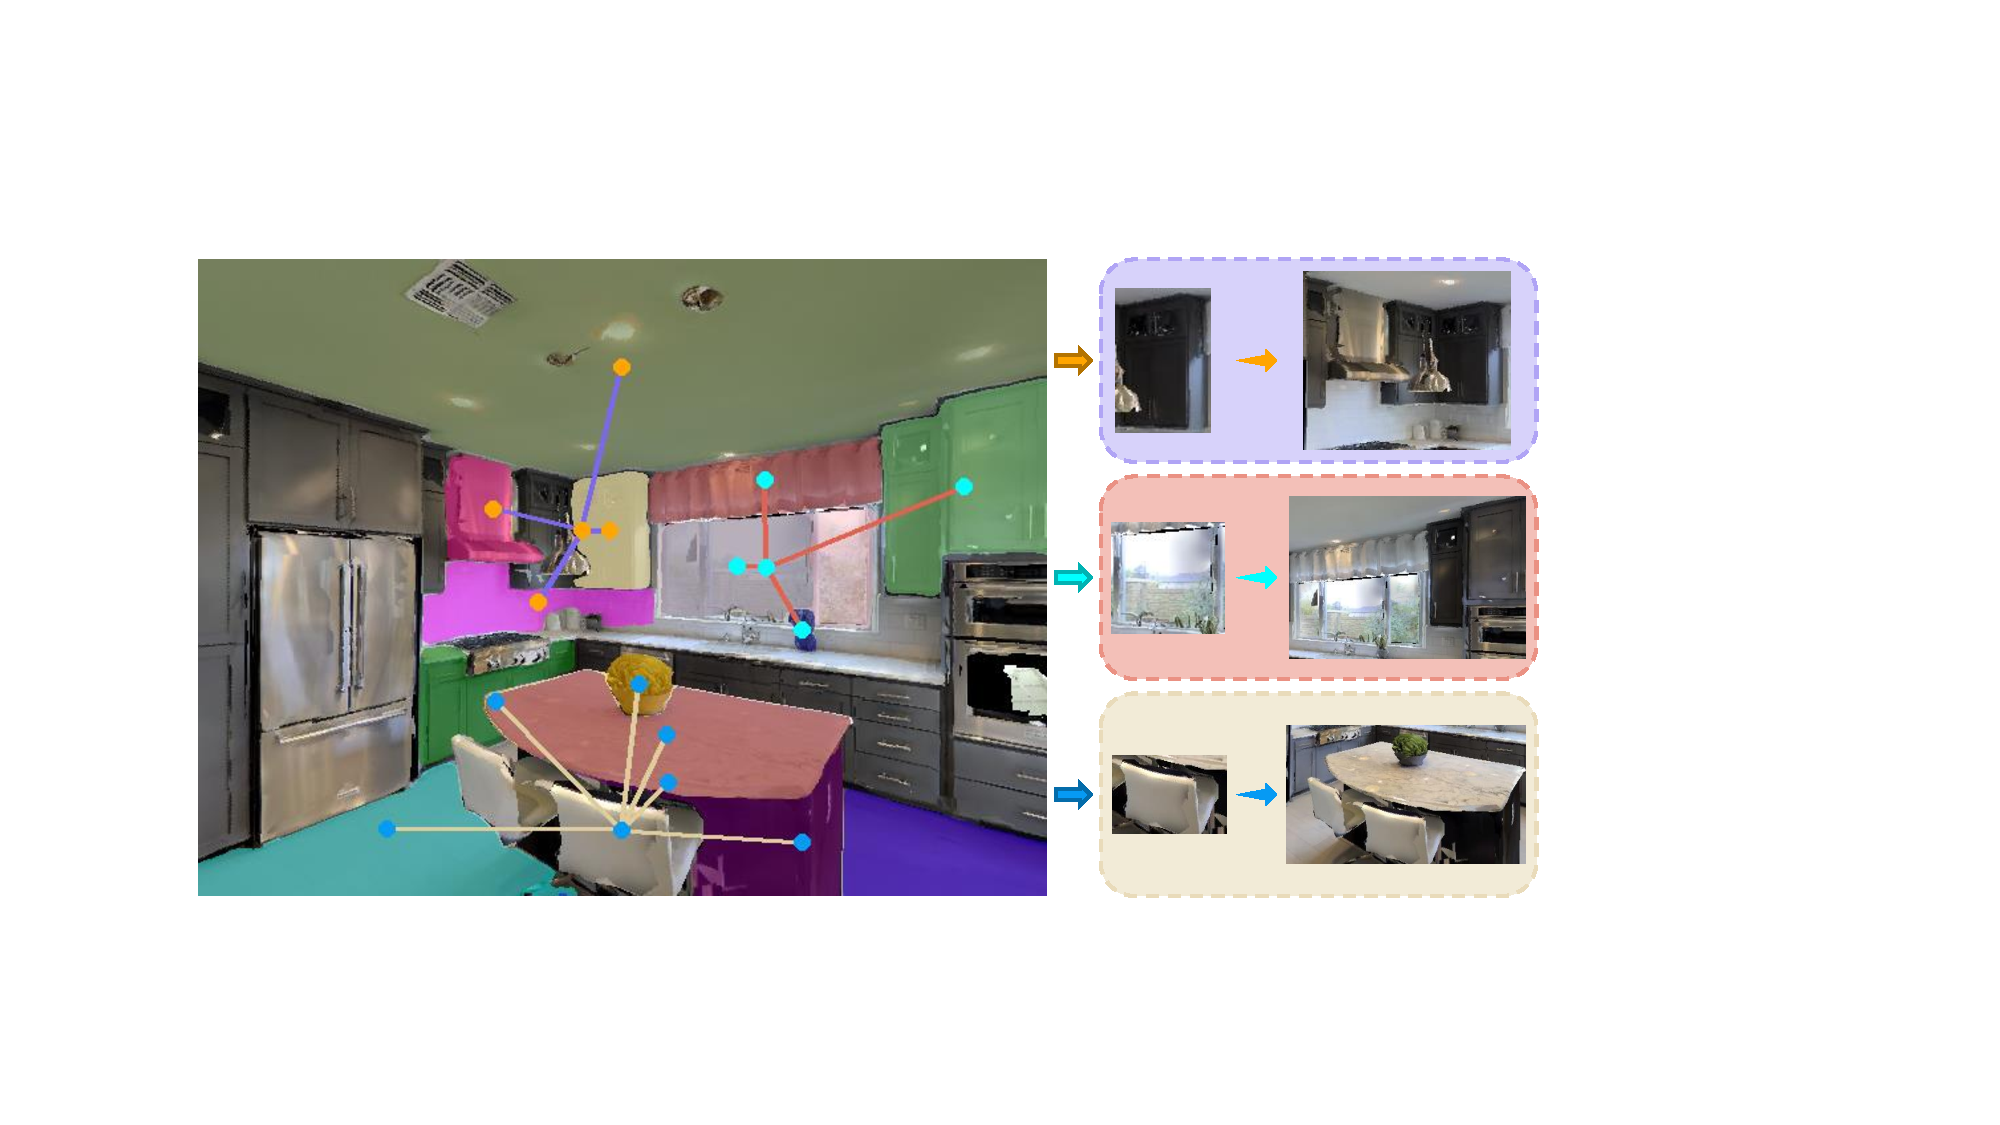
\includegraphics[width=\columnwidth]{expander.pdf}
    \vspace{-20pt}
    \caption{感受野扩展器将感受野从单个物体扩展到富含上下文信息的区域。通过利用物体邻接矩阵和每个物体的边界框,它将单个物体如橱柜、窗户玻璃和椅子扩展为物体区域,如模块化厨房、多窗玻璃和餐桌套件,分别。}
    \vspace{-5pt}
    \label{fig:expander_image}
\end{figure}

给定图像中的物体邻接矩阵和边界框,对于每一个物体,我们考虑其邻接物体的边界框,并将当前物体的边界框扩展,以包含所有邻接物体。这种扩展增加了感受野,使我们能够捕捉更丰富的上下文信息,如 \fref{fig:expander_image} 所示。随后我们应用非极大值抑制(Non-Maximum Suppression,NMS),选取置信度最高的边界框,并基于其交并比(IoU)分数移除重叠边界框,从而获得一组干净且信息丰富的物体图像块。

\begin{figure*}[t]
    \centering
    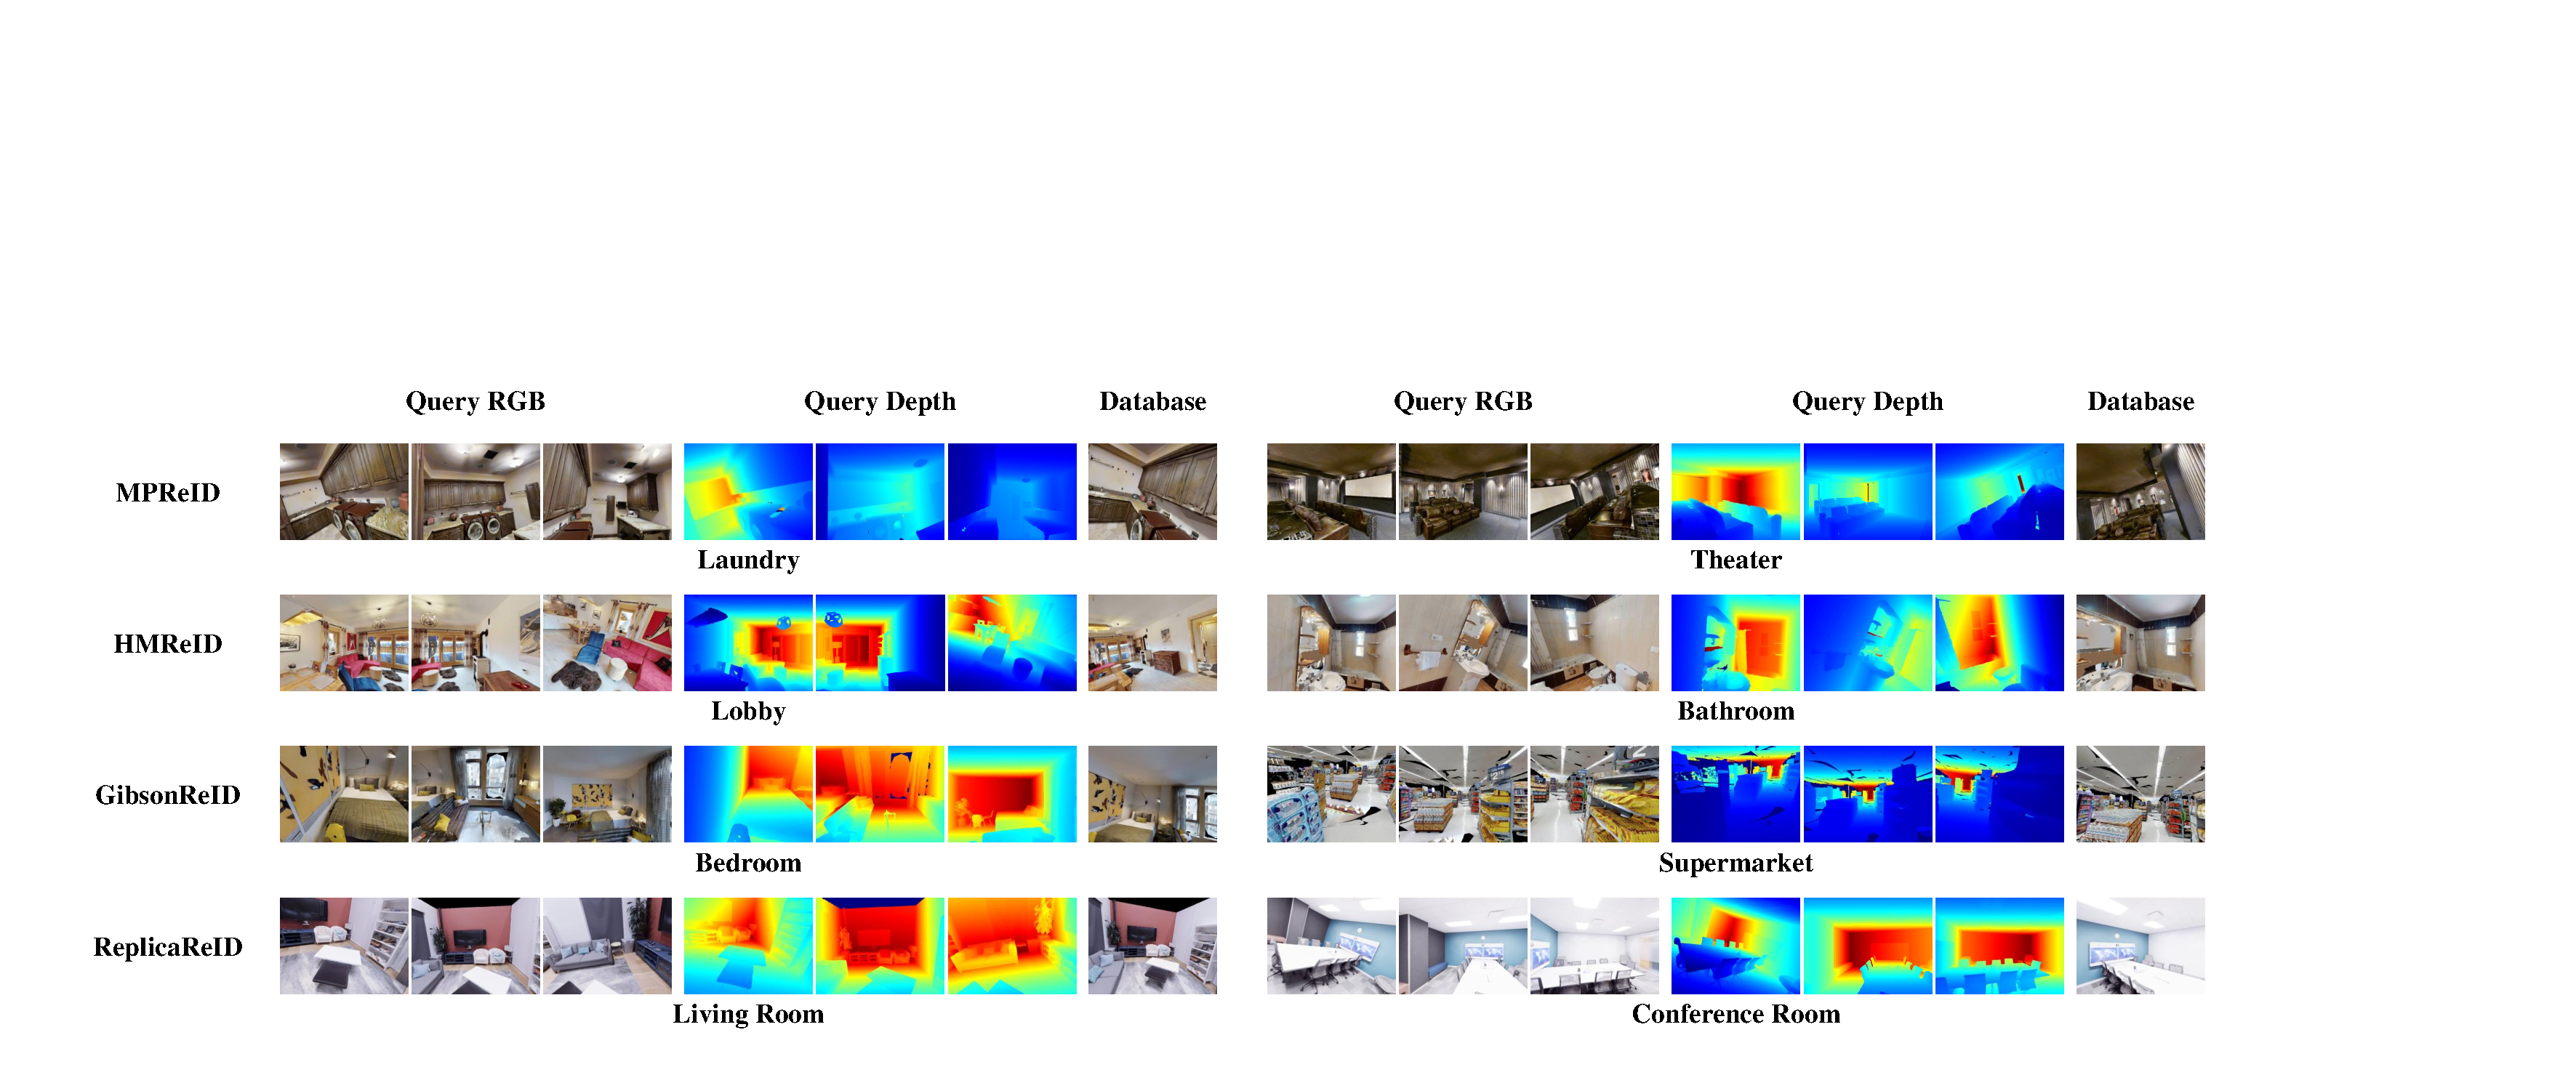
\includegraphics[width=\textwidth]{dataset_font.pdf}
    \vspace{-20pt}
    \caption{四个新构建的房间重新识别数据集示意图:MPReID、HMReID、GibsonReID 和 ReplicaReID。每个房间在数据库中仅提供一张参考图像,而查询图像则从不同视角捕捉每个房间。}
    \vspace{-10pt}
    \label{fig:dataset_image}
\end{figure*}
\subsubsection{面向对象的细化}
\label{subsec:refinement}

面向对象的细化模块由三个关键子模块组成:对象特征提取器、互近邻算法和面向对象的评分。

\vspace{-6pt}
\paragraph{对象特征提取器}

为了有效地利用对象块和对象分割信息,我们优先考虑全局特征,而不是局部特征聚合。后者方法可能无法有效捕捉对象特征,并且可能显著增加计算复杂度和存储需求 \cite{zheng2018sift}。如第~\ref{sec:section3.1.1}节所讨论的,我们继续依赖于在大规模图像数据集上预训练的模型。使用对象特征提取器,我们可以获得查询块和参考块及对象的特征。设\(Q_p=\{\mathbf{p_i^q}\}_{i=1}^{n_{qp}}\)和\(Q_o=\{\mathbf{o_i^q}\}_{i=1}^{n_{qo}}\)分别表示查询块和对象的特征集。对于查询的五个\mbox{候选}参考图像,我们将参考块和对象的特征集定义为\(R_p=\{\mathbf{p_i^r}\}_{i=1}^{n_{rp}}\)和\(R_o=\{\mathbf{o_i^r}\}_{i=1}^{n_{ro}}\)。

\vspace{-6pt}
\paragraph{互近邻算法} 给定一组查询特征\(\{\mathbf{f_i^q}\}_{i=1}^{n_q}\)和参考特征\(\{\mathbf{f_i^r}\}_{i=1}^{n_r}\),通过对两个特征集进行穷举比较,识别出互近邻匹配对。设\(P\)表示这些互近邻匹配对的余弦相似度得分集,则有
\begin{equation}
    P = \{\cos(\mathbf{f_i^q}, \mathbf{f_j^r}) \mid i = \text{NN}_r(\mathbf{f_j^r}), \; j = \text{NN}_q(\mathbf{f_i^q})\}
    \label{eq:mutual nearest neighbors}
\end{equation}
其中
\begin{equation}
    \text{NN}_q(\mathbf{f_i^q}) = \arg\max_{j} \left( \frac{\mathbf{f_i^q} \cdot \mathbf{f_j^r}}{\|\mathbf{f_i^q}\| \|\mathbf{f_j^r}\|} \right),
\end{equation}
\begin{equation}
    \text{NN}_r(\mathbf{f_i^r}) = \arg\max_{j} \left( \frac{\mathbf{f_i^r} \cdot \mathbf{f_j^q}}{\|\mathbf{f_i^r}\| \|\mathbf{f_j^q}\|} \right),
\end{equation}
\begin{equation}
    \cos(\mathbf{f_i^q}, \mathbf{f_j^r}) = \frac{\mathbf{f_i^q} \cdot \mathbf{f_j^r}}{\|\mathbf{f_i^q}\| \|\mathbf{f_j^r}\|}.
\end{equation}
通过利用互近邻算法,我们可以显著提高检索准确性,同时缩小搜索空间并提高整体检索效率 \cite{zhong2017reranking}。

\vspace{-6pt}
\paragraph{面向对象的评分} 面向对象的得分\(s\)是全局得分\(s_{\text{global}}\)(在方程~\ref{eq:global feature cosine similarity}中计算)、块得分\(s_{\text{patch}}\)和对象得分\(s_{\text{object}}\)的和:
\begin{equation}
    s = s_{\text{global}} + s_{\text{patch}}(Q_p, R_p) + s_{\text{object}}(Q_o, R_o).
    \label{eq:object-aware scoring}
\end{equation}
其中,\(s_{\text{patch}}\)和\(s_{\text{object}}\)可以是\(s_{\text{mean}}\)或\(s_{\max}\),其中
\begin{subequations}
\begin{align}
    s_{\text{mean}}(Q_t, R_t) &= \frac{1}{|P(Q_t, R_t)|} \sum_{x \in P(Q_t, R_t)} x,
    \label{eq:mean}\\
    s_{\max}(Q_t, R_t) &= \max_{x \in P(Q_t, R_t)} x.
    \label{eq:max}
\end{align}
\end{subequations}
在这些方程中,\(P\)表示互近邻匹配对的余弦相似度得分集,\(Q_t\)表示\(Q_p\)或\(Q_o\),而\(R_t\)表示\(R_p\)或\(R_o\)。全局得分\(s_{\text{global}}\)作为先验,表明初始的五个候选具有不同的相关性。因此,我们保留这一项以考虑它们的不同相关性。

\vspace{-8pt}
\paragraph{面向对象的细化} 对于每个查询,我们使用面向对象的评分从初始的五个候选中选择最相似的前两个参考候选:
\begin{equation}
    \text{Top}_2(\mathbf{s}_{i}) = \text{argsort}(-\mathbf{s}_{i})[:2],
\end{equation}
其中,\(\mathbf{s}_{i}\)是第\(i\)个查询的面向对象的得分。
\subsection{细粒度阶段}

补丁和物体特征为理解房间布局提供了有价值的信息;然而,在区分高度视觉相似的房间时,尤其是在视角变化和遮挡存在的情况下,它们可能不足以提供足够的区分度。与此相比,物体上的关键点表现出对纹理和外观变化的强大鲁棒性,使其能够有效地处理部分遮挡并排除异常值 \cite{1498756}。这使得关键点能够提供一种更精细的方法,捕捉更细致的细节,从而实现更精确的房间识别。在此阶段,我们使用细粒度检索来选择最终的 top-1 结果。
\subsubsection{细粒度检索}

深度匹配器,如 SuperGlue \cite{sarlin2020supergluelearningfeaturematching},在室内外的挑战性条件下,在视觉定位任务中表现良好。然而,它们通常面临效率问题。相比之下,LightGlue \cite{lindenberger2023lightgluelocalfeaturematching} 提供了高效性,并且没有牺牲匹配准确性,使其成为我们细粒度检索的理想选择。

对于每个查询图像及其两个候选参考图像,我们将查询图像与每个候选图像进行匹配,并记录匹配的关键点对数量。更多的匹配通常意味着两张图像的特征之间有更大的重叠和一致性,表明它们内容的相似度较高 \cite{Lowe2004DistinctiveIF}。具有更多匹配的候选图像被选为最终结果。
